\documentclass[aspectratio=169, table, 12pt]{beamer}

\usepackage{colortbl}
\usepackage{xcolor}
\usepackage{listings}
\usepackage{tabularx}
\usepackage{tikz}
\usetikzlibrary{arrows.meta, positioning, calc, fit, shapes.geometric}

\makeatletter
\def\input@path{{../theme/}}
\makeatother
\graphicspath{{../theme/}{../../figures/}}
\usetheme{Pradita}

\definecolor{praditagreen}{RGB}{37, 113, 71}

% Tema membuat garis tabel berwarna putih. Dikembalikan agar tabel terbaca.
\arrayrulecolor{black}
\setlength{\arrayrulewidth}{0.5pt}

% Kolom X rata kiri, dipakai pada tabel dengan kolom X yang sempit, agar
% spasi antarkata tidak meregang.
\newcolumntype{Y}{>{\raggedright\arraybackslash}X}

\lstdefinelanguage{bash}{
  keywords={},
  basicstyle=\ttfamily\scriptsize,
  ndkeywords={cd, python3, google-chrome},
  ndkeywordstyle=\color{purple}\bfseries,
  sensitive=true,
  commentstyle=\color{gray},
  numbers=none,
  breaklines=true,
  frame=lines,
  backgroundcolor=\color{lightgray!10},
  tabsize=2,
  comment=[l]{\#},
  showstringspaces=false
}

\lstdefinelanguage{TypeScript}{
  keywords={const, let, function, return, async, await, try, catch, throw,
            new, if, for, of},
  ndkeywords={Promise, caches, fetch, self},
  basicstyle=\ttfamily\scriptsize,
  keywordstyle=\color{blue}\bfseries,
  ndkeywordstyle=\color{purple}\bfseries,
  sensitive=true,
  commentstyle=\color{gray}\itshape,
  stringstyle=\color{red},
  numbers=none,
  breaklines=true,
  frame=lines,
  backgroundcolor=\color{lightgray!10},
  tabsize=2,
  comment=[l]{//},
  morestring=[b]",
  showstringspaces=false
}

% Gaya Python disamakan dengan naskah bab, tanpa nomor baris.
\lstdefinestyle{PythonStyle}{
  language=Python,
  basicstyle=\ttfamily\scriptsize,
  morekeywords={with, as, yield, async, await, match, case},
  keywordstyle=\color{blue}\bfseries,
  emph={math, time, json},
  emphstyle=\color{purple}\bfseries,
  commentstyle=\color{gray}\itshape,
  stringstyle=\color{red},
  numbers=none,
  breaklines=true,
  frame=lines,
  backgroundcolor=\color{lightgray!10},
  tabsize=2,
  showstringspaces=false
}

\title{\Huge Skalabilitas dan\\ \vspace{10pt} Emerging Web}
\subtitle{IF140303 - Pengembangan Aplikasi Web}
\author{\textbf{Alfa Yohannis}}

\begin{document}

\frame{\titlepage}

\begin{frame}[fragile]
  \frametitle{Isi Pertemuan}
  \vspace{14pt}
  \begin{columns}[t]
    \column{0.5\textwidth}
    {\small\tableofcontents[sections={1-7}]}

    \column{0.5\textwidth}
    {\small\tableofcontents[sections={8-13}]}
  \end{columns}
\end{frame}

\begin{frame}{\hfill}
  \centering
  \Huge{\textbf{Apa yang terjadi bila\\bebannya naik 100 kali lipat?}}
\end{frame}

\section{Tujuan dan Kerangka Bahasan}

\begin{frame}{\hfill}
  \centering
  \Huge{\textbf{Tujuan dan Kerangka Bahasan}}
\end{frame}

\begin{frame}{{\Large Tujuan Pembelajaran}}
  \vspace{10pt}
  \begin{itemize}
    \item Mengukur penskalaan horizontal sampai satu komponen bersama menjadi
          \textit{bottleneck}, lalu menunjukkan pergeseran
          \textit{bottleneck}-nya dari angka.
    \item Merancang rencana kapasitas untuk beban 100 kali lipat yang
          mencakup batas layanan, replikasi, partisi, dan biaya.
    \item Membandingkan mode \textit{offline} Progressive Web App (PWA),
          \textit{cold start} \textit{serverless}, dan fitur berbantuan Large
          Language Model (LLM) berdasarkan hasil pengukuran.
  \end{itemize}
\end{frame}

\begin{frame}{{\Large Dua Jawaban Cepat yang Menyesatkan}}
  \vspace{12pt}
  \begin{itemize}
    \item Membeli server yang lebih besar ada batasnya, dan satu proses
          Python yang terkunci Global Interpreter Lock (GIL) tidak memakai
          core tambahan.
    \item Memecah aplikasi menjadi banyak layanan menambah jaringan di antara
          bagian yang dahulu cukup saling memanggil.
  \end{itemize}
  \vspace{10pt}
  {\small Bab ini menjawab dengan pengukuran: replika ditambah sampai satu
  komponen bersama penuh, panggilan fungsi diadu dengan panggilan
  jaringan, dua cara membagi data dibandingkan, lalu seluruhnya disusun menjadi
  satu rencana kapasitas.}
\end{frame}

\section{Penskalaan Vertikal dan Horizontal}

\begin{frame}{\hfill}
  \centering
  \Huge{\textbf{Penskalaan Vertikal\\dan Horizontal}}
\end{frame}

\begin{frame}{{\Large Replika Tanpa State, Satu Basis Data}}
  \vspace{6pt}
  \centering
  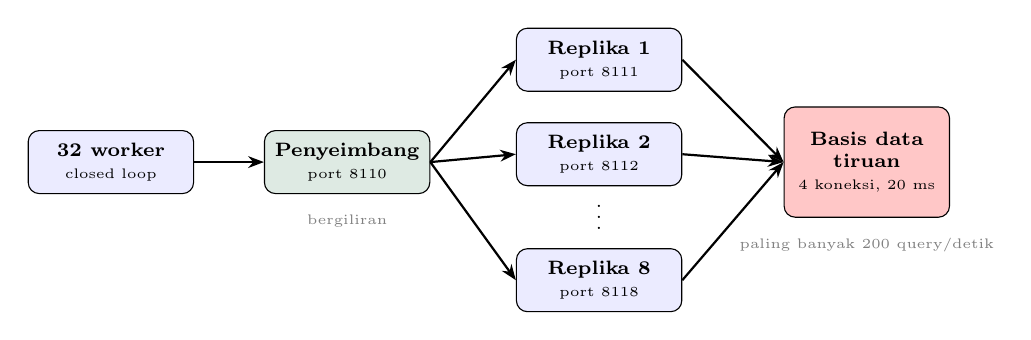
\begin{tikzpicture}[
    font=\scriptsize,
    kotak/.style={draw, rounded corners, minimum height=0.8cm,
                  minimum width=2.1cm, align=center, font=\scriptsize\bfseries},
    panah/.style={-{Stealth[length=2mm]}, thick}
  ]
    \node[kotak, fill=blue!8] (worker) at (0,0) {32 worker\\{\tiny\mdseries closed loop}};
    \node[kotak, fill=praditagreen!15] (penyeimbang) at (3.0,0) {Penyeimbang\\{\tiny\mdseries port 8110}};
    \node[kotak, fill=blue!8] (replika1) at (6.2,1.3) {Replika 1\\{\tiny\mdseries port 8111}};
    \node[kotak, fill=blue!8] (replika2) at (6.2,0.1) {Replika 2\\{\tiny\mdseries port 8112}};
    \node[kotak, fill=blue!8] (replika8) at (6.2,-1.5) {Replika 8\\{\tiny\mdseries port 8118}};
    \node at (6.2,-0.6) {$\vdots$};
    \node[kotak, fill=red!22, minimum height=1.4cm] (basisdata) at (9.6,0) {Basis data\\tiruan\\{\tiny\mdseries 4 koneksi, 20 ms}};

    \draw[panah] (worker) -- (penyeimbang);
    \draw[panah] (penyeimbang.east) -- (replika1.west);
    \draw[panah] (penyeimbang.east) -- (replika2.west);
    \draw[panah] (penyeimbang.east) -- (replika8.west);
    \draw[panah] (replika1.east) -- (basisdata.west);
    \draw[panah] (replika2.east) -- (basisdata.west);
    \draw[panah] (replika8.east) -- (basisdata.west);
    \node[font=\tiny, gray] at (3.0,-0.75) {bergiliran};
    \node[font=\tiny, gray] at (9.6,-1.05) {paling banyak 200 query/detik};
  \end{tikzpicture}

  \vspace{4pt}
  {\small Analoginya warung dengan banyak kasir yang mengambil pesanan dari
  satu dapur. Ketika dapurnya penuh, kasir tambahan hanya memindahkan antrean
  ke depan dapur.}
\end{frame}

\begin{frame}[fragile]{{\Large Komponen Bersama Berkapasitas Tetap}}
  \vspace{2pt}
\begin{lstlisting}[style=PythonStyle]
def baca_kesukaan(nomor_pengguna):
  with SLOT_KONEKSI:
    time.sleep(WAKTU_QUERY_DETIK)
  return [(nomor_pengguna + langkah * JARAK_KATEGORI) % JUMLAH_KATEGORI
          for langkah in range(KATEGORI_PER_PENGGUNA)]
\end{lstlisting}
  \vspace{2pt}
  {\small Paling banyak empat \textit{query} bersamaan, masing-masing 20
  milidetik, sehingga batas atasnya 200 \textit{query} per detik, berapa pun
  jumlah replika di depannya. Tiap replika menghitung skor 20.000 buku sekitar
  8 milidetik dengan Python murni, jadi satu replika memakai satu core.}
\end{frame}

\begin{frame}{{\Large Satu sampai Delapan Replika, Diukur}}
  \vspace{6pt}
  \centering
  {\footnotesize
  \begin{tabularx}{\textwidth}{Yllll}
    \hline
    \textbf{Replika} & \textbf{Per detik} & \textbf{p50 ms} & \textbf{p95 ms} & \textbf{Efisiensi} \\
    \hline
    1 & 106,8 & 286,1 & 547,5 & 100\% \\
    \hline
    2 & 186,6 & 161,4 & 278,3 & 87\% \\
    \hline
    4 & 198,2 & 161,4 & 168,6 & 46\% \\
    \hline
    8 & 198,0 & 161,4 & 168,9 & 23\% \\
    \hline
  \end{tabularx}}

  \vspace{6pt}
  {\small Dari empat ke delapan replika, \textit{throughput} tidak bergerak:
  198,2 lalu 198,0. Bagian yang tidak ikut bertambah menentukan batas seluruh
  sistem, persis seperti hukum Amdahl.}
\end{frame}

\begin{frame}{{\Large Dihitung Sebelum Diukur}}
  \vspace{12pt}
  \begin{itemize}
    \item Hukum Little: 32 \textit{worker} dibagi 198,2 permintaan per detik
          sama dengan 0,161 detik. Yang terukur: p50 161,4 ms pada empat
          maupun delapan replika.
    \item Nilai p95 satu replika 547,5 ms, hampir dua kali p50-nya, karena
          32 permintaan berebut satu proses dan giliran GIL tidak adil.
    \item Begitu antreannya pindah ke basis data, antrean berjalan berurutan
          dan p95 merapat ke p50: 168,6 lawan 161,4.
  \end{itemize}
\end{frame}

\begin{frame}{{\Large Bottleneck yang Pindah}}
  \vspace{6pt}
  \centering
  {\footnotesize
  \begin{tabularx}{\textwidth}{Ylll}
    \hline
    \textbf{Replika, 16 koneksi} & \textbf{Per detik} & \textbf{p50 ms} & \textbf{Efisiensi} \\
    \hline
    1 & 105,0 & 288,9 & 100\% \\
    \hline
    2 & 179,8 & 169,5 & 86\% \\
    \hline
    4 & 285,0 & 105,2 & 68\% \\
    \hline
    8 & 347,8 & 87,4 & 41\% \\
    \hline
  \end{tabularx}}

  \vspace{6pt}
  {\small Batas basis data naik menjadi 800 \textit{query} per detik, tetapi
  delapan replika hanya bekerja 41\%. Laptop Intel Core i9-11900H mencapai 4,9
  GHz bila satu core bekerja dan melambat bila semuanya bekerja.
  \textit{Bottleneck} tidak hilang, hanya pindah.}
\end{frame}

\section{Modular Monolith dan Microservices}

\begin{frame}{\hfill}
  \centering
  \Huge{\textbf{Modular Monolith\\dan Microservices}}
\end{frame}

\begin{frame}{{\Large Satu Kebutuhan, Dua Bentuk}}
  \vspace{6pt}
  \centering
  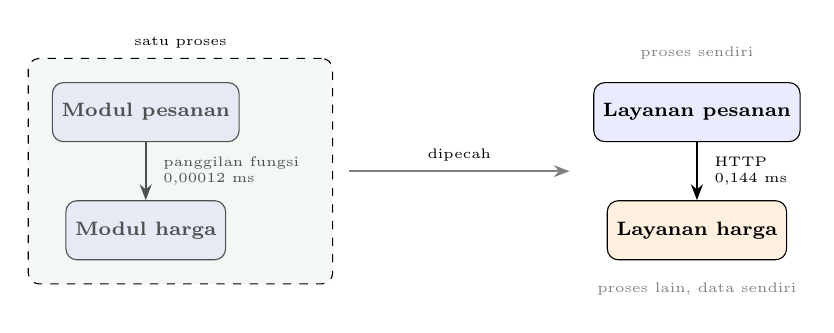
\begin{tikzpicture}[
    font=\scriptsize,
    kotak/.style={draw, rounded corners, minimum height=0.75cm,
                  minimum width=1.9cm, align=center, font=\scriptsize\bfseries},
    panah/.style={-{Stealth[length=2mm]}, thick}
  ]
    \node[kotak, fill=blue!8] (pesanan1) at (0,0.6) {Modul pesanan};
    \node[kotak, fill=blue!8] (harga1) at (0,-0.9) {Modul harga};
    \draw[panah] (pesanan1) -- (harga1);
    \node[font=\tiny, align=left, anchor=west] (catatan1) at (0.1,-0.15) {panggilan fungsi\\0,00012 ms};
    \node[draw, dashed, rounded corners, fill=praditagreen!15, fill opacity=0.35, text opacity=1,
          fit=(pesanan1)(harga1)(catatan1), inner sep=0.3cm,
          label={[font=\tiny]above:satu proses}] (proses) {};

    \node[kotak, fill=blue!8] (pesanan2) at (7.0,0.6) {Layanan pesanan};
    \node[kotak, fill=orange!12] (harga2) at (7.0,-0.9) {Layanan harga};
    \draw[panah] (pesanan2) -- (harga2);
    \node[font=\tiny, align=left, anchor=west] at (7.1,-0.15) {HTTP\\0,144 ms};
    \node[font=\tiny, gray] at (7.0,1.35) {proses sendiri};
    \node[font=\tiny, gray] at (7.0,-1.65) {proses lain, data sendiri};

    \draw[panah, gray] ([xshift=0.2cm]proses.east) -- node[font=\tiny, above, black] {dipecah} ($(pesanan2.west |- proses.east) + (-0.3,0)$);
  \end{tikzpicture}

  \vspace{4pt}
  {\small Analoginya kantor fakultas: menoleh ke meja sebelah lawan mengirim
  kurir ke gedung lain. Kurirnya cepat, tetapi tetap jauh lebih lambat, dan
  sesekali tidak kembali.}
\end{frame}

\begin{frame}{{\Large Sepuluh Panggilan Harga, Diukur}}
  \vspace{6pt}
  \centering
  {\footnotesize
  \begin{tabularx}{\textwidth}{Ylll}
    \hline
    \textbf{Cara} & \textbf{p50 ms} & \textbf{p95 ms} & \textbf{Kali lipat} \\
    \hline
    fungsi di dalam proses & 0,0012 & 0,0012 & 1 \\
    \hline
    HTTP, sambungan dipakai ulang & 1,4436 & 1,8988 & 1.225 \\
    \hline
    HTTP, sambungan baru tiap kali & 3,1831 & 3,8629 & 2.701 \\
    \hline
  \end{tabularx}}

  \vspace{6pt}
  {\small Seluruhnya di 127.0.0.1, jaringan terbaik yang mungkin. Kolom kali
  lipat berubah jauh antarpengukuran karena penyebutnya amat kecil. Yang tetap
  adalah ordenya: ribuan kali.}
\end{frame}

\begin{frame}{{\Large Mengapa Tetap Dipecah}}
  \vspace{12pt}
  \begin{itemize}
    \item Tiap layanan di-\textit{deploy} dan diskalakan sendiri: rencana
          kapasitas bab ini membutuhkan 19 replika katalog, tetapi hanya 4
          replika akun.
    \item Harganya bukan hanya waktu. Panggilan jaringan dapat gagal
          sebagian, dan sepuluh panggilan dengan peluang lambat 1\% berpeluang
          9,6\% terkena setidaknya satu.
    \item Mulai dari \textit{monolith} yang modular, lalu pindahkan satu modul
          hanya bila ada alasan terukur, lewat \textit{reverse proxy} atau
          \textit{gateway}.
  \end{itemize}
\end{frame}

\section{Batas Layanan dan Trade-off}

\begin{frame}{\hfill}
  \centering
  \Huge{\textbf{Batas Layanan\\dan Trade-off}}
\end{frame}

\begin{frame}{{\Large Satu Istilah, Tiga Arti}}
  \vspace{6pt}
  \centering
  {\footnotesize
  \begin{tabularx}{\textwidth}{lYY}
    \hline
    \textbf{Layanan} & \textbf{Arti "buku"} & \textbf{Data yang dimilikinya} \\
    \hline
    katalog & judul yang dicari dan dibaca & judul, sinopsis, harga tayang \\
    \hline
    pesanan & baris pesanan yang dibayar & harga saat dibeli, jumlah, status \\
    \hline
    akun & riwayat milik seorang pengguna & daftar keinginan, ulasan \\
    \hline
  \end{tabularx}}

  \vspace{6pt}
  {\small Batas layanan mengikuti batas makna, yang disebut \textit{bounded
  context}, bukan batas tabel. Sistem juga cenderung meniru jalur komunikasi
  tim yang membuatnya.}
\end{frame}

\begin{frame}{{\Large Pilihan Menurut CAP dan PACELC}}
  \vspace{6pt}
  \centering
  {\footnotesize
  \begin{tabularx}{\textwidth}{llY}
    \hline
    \textbf{Keadaan jaringan} & \textbf{Yang dipilih} & \textbf{Akibat bagi pengguna} \\
    \hline
    terputus & konsistensi & tulisan ditolak atau ditunda sampai pulih \\
    \hline
    terputus & ketersediaan & tulisan diterima, \textit{conflict} diselesaikan kemudian \\
    \hline
    normal & \textit{latency} & dibaca dari replika terdekat, mungkin \textit{stale} \\
    \hline
    normal & konsistensi & dibaca dari \textit{primary}, lebih lambat \\
    \hline
  \end{tabularx}}

  \vspace{6pt}
  {\small CAP (Consistency, Availability, Partition tolerance) untuk dua baris
  pertama, PACELC untuk dua baris terakhir. Stok saat pembayaran memilih
  konsistensi, katalog memilih ketersediaan.}
\end{frame}

\section{Partisi dan Rencana Kapasitas}

\begin{frame}{\hfill}
  \centering
  \Huge{\textbf{Partisi dan\\Rencana Kapasitas}}
\end{frame}

\begin{frame}{{\Large Lingkaran Hash}}
  \vspace{6pt}
  \centering
  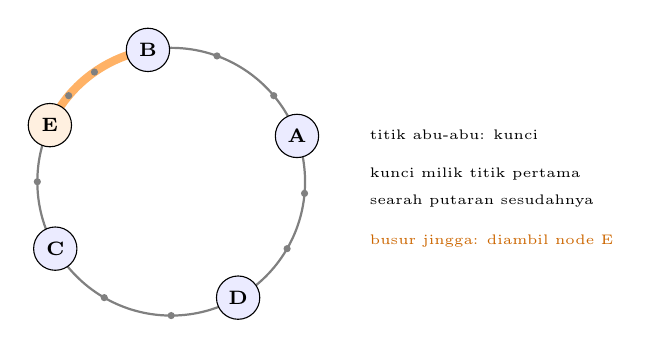
\begin{tikzpicture}[
    font=\scriptsize,
    titik/.style={circle, draw, minimum size=0.55cm, inner sep=0pt, font=\scriptsize\bfseries},
    panah/.style={-{Stealth[length=2mm]}, thick}
  ]
    \draw[thick, gray] (0,0) circle (1.7cm);
    \draw[line width=3pt, orange!60] (100:1.7cm) arc (100:155:1.7cm);
    \node[titik, fill=blue!8] at (20:1.7cm) {A};
    \node[titik, fill=blue!8] at (100:1.7cm) {B};
    \node[titik, fill=blue!8] at (210:1.7cm) {C};
    \node[titik, fill=blue!8] at (300:1.7cm) {D};
    \node[titik, fill=orange!12] at (155:1.7cm) {E};
    \foreach \sudut in {40, 70, 125, 140, 180, 240, 270, 330, 355} {
      \fill[gray] (\sudut:1.7cm) circle (1.3pt);
    }
    \node[font=\tiny, align=left, anchor=west] at (2.4,0.6) {titik abu-abu: kunci};
    \node[font=\tiny, align=left, anchor=west] at (2.4,0.1) {kunci milik titik pertama};
    \node[font=\tiny, align=left, anchor=west] at (2.4,-0.25) {searah putaran sesudahnya};
    \node[font=\tiny, align=left, anchor=west, orange!80!black] at (2.4,-0.75) {busur jingga: diambil node E};
  \end{tikzpicture}

  \vspace{4pt}
  {\small Modulo seperti loket uang kuliah yang dibagi menurut sisa bagi nomor
  induk: membuka loket kelima memindahkan hampir semua mahasiswa.
  \textit{Consistent hashing} hanya memindahkan kunci di busur
  \textit{node} baru.}
\end{frame}

\begin{frame}{{\Large Empat Node Menjadi Lima, Dihitung}}
  \vspace{6pt}
  \centering
  {\footnotesize
  \begin{tabularx}{\textwidth}{Ylll}
    \hline
    \textbf{Cara} & \textbf{Kunci pindah} & \textbf{Terberat, kunci} & \textbf{Terberat, permintaan} \\
    \hline
    modulo & 80,2\% & 20,2\% & 24,3\% \\
    \hline
    \textit{consistent hashing}, 1 titik & 2,1\% & 49,2\% & 43,3\% \\
    \hline
    \textit{consistent hashing}, 100 titik & 20,2\% & 21,2\% & 26,9\% \\
    \hline
  \end{tabularx}}

  \vspace{6pt}
  {\small Satu titik per \textit{node} hanya memindahkan 2,1\%, dan itu tanda
  buruk: satu \textit{node} lama memegang 49,2\% kunci. Pelanggan teratas
  membawa sekitar 8,3\% permintaan, berapa pun cara baginya.}
\end{frame}

\begin{frame}[fragile]{{\Large Inti Rencana Kapasitas}}
  \vspace{2pt}
\begin{lstlisting}[style=PythonStyle]
  replika = math.ceil(target_rps / budget_replika_rps)
  shard = max(1, math.ceil(tulis_qps / budget_node_qps))
  replika_baca_per_shard = math.ceil(baca_qps / shard / budget_node_qps)
  node_basis_data = shard * (1 + replika_baca_per_shard)
\end{lstlisting}
  \vspace{4pt}
  {\small Tiap \textit{budget} hanya 60\% dari kapasitas terukur, yaitu 106,8
  permintaan per detik per replika dan 198,2 \textit{query} per detik per
  \textit{node}. Replika baca menolong pembacaan, sedangkan tulisan yang
  melebihi satu \textit{node} harus dipartisi.}
\end{frame}

\begin{frame}{{\Large Rencana untuk Beban 100 Kali Lipat}}
  \vspace{6pt}
  \centering
  {\footnotesize
  \begin{tabularx}{\textwidth}{Yllllll}
    \hline
    \textbf{Layanan} & \textbf{Target/s} & \textbf{Replika} & \textbf{Baca/s} & \textbf{Tulis/s} & \textbf{\textit{Node} data} & \textbf{Juta Rp} \\
    \hline
    katalog & 1.200 & 19 & 235,2 & 48,0 & 3 & 9,3 \\
    \hline
    pesanan & 300 & 5 & 360,0 & 540,0 & 10 & 13,5 \\
    \hline
    akun & 200 & 4 & 90,0 & 20,0 & 2 & 3,6 \\
    \hline
    \textbf{Jumlah} & & \textbf{28} & & & \textbf{15} & \textbf{26,4} \\
    \hline
  \end{tabularx}}

  \vspace{6pt}
  {\small Pesanan butuh lima \textit{shard} karena 540 tulisan per detik
  melebihi 118,9. Tanpa \textit{cache}, katalog butuh 21 \textit{node} dan
  biayanya naik ke Rp 48,0 juta. Biaya per \textit{node} hanya asumsi
  contoh.}
\end{frame}

\section{Multi-Region dan Edge Computing}

\begin{frame}{\hfill}
  \centering
  \Huge{\textbf{Multi-Region dan\\Edge Computing}}
\end{frame}

\begin{frame}{{\Large Jarak Tidak Dapat Ditawar dengan Kode}}
  \vspace{6pt}
  \centering
  {\footnotesize
  \begin{tabularx}{\textwidth}{Ylll}
    \hline
    \textbf{Wilayah server} & \textbf{Jarak} & \textbf{RTT minimum} & \textbf{Tiga RTT} \\
    \hline
    Singapura & 905 km & 9,1 ms & 27,2 ms \\
    \hline
    Tokyo & 5.782 km & 57,8 ms & 173,5 ms \\
    \hline
    Frankfurt & 11.119 km & 111,2 ms & 333,6 ms \\
    \hline
    Virginia, Amerika Serikat & 16.338 km & 163,4 ms & 490,1 ms \\
    \hline
  \end{tabularx}}

  \vspace{6pt}
  {\small Dihitung dari Jakarta dengan cahaya di serat optik sekitar 200.000
  km per detik. Sambungan HTTP terenkripsi yang baru butuh tiga Round-Trip
  Time (RTT): TCP, TLS 1.3, lalu permintaannya.}
\end{frame}

\begin{frame}{{\Large Gudang Cabang dan Kode di Edge}}
  \vspace{12pt}
  \begin{itemize}
    \item \textit{Multi-region} seperti gudang cabang: pengiriman lebih
          cepat, tetapi stok tersebar dan harus dicocokkan.
    \item Sebagian barang tidak boleh keluar wilayahnya: UU PDP mengatur
          pengiriman data pribadi ke luar wilayah hukum Indonesia.
    \item \textit{Edge computing} menjalankan kode di dekat pengguna, tetapi
          fungsi yang butuh basis data di Virginia tetap membayar 163,4 ms
          tiap pertanyaan.
  \end{itemize}
\end{frame}

\section{PWA dan Offline-First}

\begin{frame}{\hfill}
  \centering
  \Huge{\textbf{PWA dan Offline-First}}
\end{frame}

\begin{frame}{{\Large Service Worker di Tengah Jalan}}
  \vspace{6pt}
  \centering
  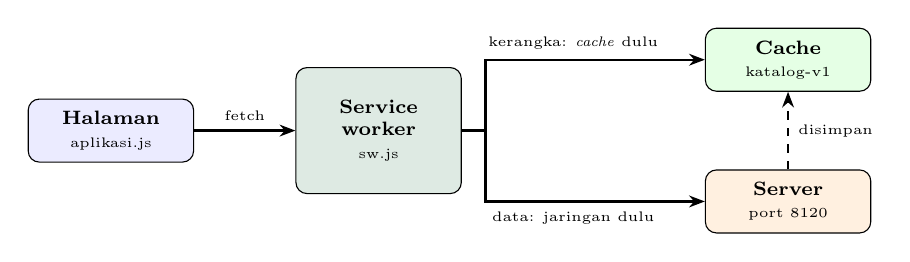
\begin{tikzpicture}[
    font=\scriptsize,
    kotak/.style={draw, rounded corners, minimum height=0.8cm,
                  minimum width=2.1cm, align=center, font=\scriptsize\bfseries},
    panah/.style={-{Stealth[length=2mm]}, thick}
  ]
    \node[kotak, fill=blue!8] (halaman) at (0,0) {Halaman\\{\tiny\mdseries aplikasi.js}};
    \node[kotak, fill=praditagreen!15, minimum height=1.6cm] (sw) at (3.4,0) {Service\\worker\\{\tiny\mdseries sw.js}};
    \node[kotak, fill=green!10] (cache) at (8.6,0.9) {Cache\\{\tiny\mdseries katalog-v1}};
    \node[kotak, fill=orange!12] (server) at (8.6,-0.9) {Server\\{\tiny\mdseries port 8120}};

    \draw[panah] (halaman) -- node[font=\tiny, above] {fetch} (sw);
    \draw[panah] (sw.east) -- ++(0.3,0) |- node[font=\tiny, above, pos=0.7] {kerangka: \textit{cache} dulu} (cache.west);
    \draw[panah] (sw.east) -- ++(0.3,0) |- node[font=\tiny, below, pos=0.7] {data: jaringan dulu} (server.west);
    \draw[panah, dashed] (server.north) -- node[font=\tiny, right] {disimpan} (cache.south);
  \end{tikzpicture}

  \vspace{4pt}
  {\small Analoginya petugas loket yang menyimpan \textit{copy} daftar buku di
  laci: ketika sistem pusat \textit{down}, daftar terakhir tetap dapat ditunjukkan,
  lengkap dengan tanggalnya.}
\end{frame}

\begin{frame}[fragile]{{\Large Jaringan Dulu, Copy Bila Gagal}}
  \vspace{2pt}
\begin{lstlisting}[language=TypeScript]
async function jaringanLebihDahulu(permintaan) {
  const cache = await caches.open(NAMA_CACHE);
  try {
    const respon = await fetch(permintaan);
    await cache.put(permintaan, respon.clone());
    return respon;
  } catch (gagal) {
    const tersimpan = await cache.match(permintaan);
    if (!tersimpan) {
      throw gagal;
    }
    return tandaiDariCache(tersimpan);
  }
}
\end{lstlisting}
\end{frame}

\begin{frame}{{\Large Empat Kunjungan, Diukur}}
  \vspace{6pt}
  \centering
  {\footnotesize
  \begin{tabularx}{\textwidth}{Ylllll}
    \hline
    \textbf{Kunjungan} & \textbf{Server} & \textbf{Buku} & \textbf{Sumber} & \textbf{Tampil ms} & \textbf{Ke server} \\
    \hline
    1, profil baru & hidup & 8 & jaringan & 377 & 11 \\
    \hline
    2, profil sama & hidup & 8 & jaringan & 62 & 2 \\
    \hline
    3, profil sama & \textit{down} & 8 & \textit{cache} & 31 & 0 \\
    \hline
    4, profil baru & \textit{down} & 0 & gagal & - & 0 \\
    \hline
  \end{tabularx}}

  \vspace{6pt}
  {\small \textit{Service worker} hanya melindungi pengguna yang pernah datang.
  Dua permintaan pada kunjungan kedua adalah data katalog dan navigasi yang
  dikirim Chrome bersamaan dengan menyalakan \textit{service worker}.}
\end{frame}

\section{WebAssembly dan Serverless}

\begin{frame}{\hfill}
  \centering
  \Huge{\textbf{WebAssembly dan Serverless}}
\end{frame}

\begin{frame}{{\Large Kapan WebAssembly Layak Dipakai}}
  \vspace{6pt}
  \centering
  {\footnotesize
  \begin{tabularx}{\textwidth}{YY}
    \hline
    \textbf{Layak} & \textbf{Tidak layak} \\
    \hline
    perhitungan berat di browser, misalnya pengolahan gambar atau video & mengubah DOM, mengisi form, menangani klik \\
    \hline
    membawa pustaka C, C++, atau Rust yang sudah teruji & logika bisnis yang cukup ditulis dengan JavaScript \\
    \hline
    pekerjaan yang sama di browser dan di server & halaman yang harus tampil secepat mungkin pada kunjungan pertama \\
    \hline
  \end{tabularx}}

  \vspace{6pt}
  {\small Wasm tidak menyentuh Document Object Model (DOM) secara langsung, dan
  modulnya harus diunduh serta dikompilasi sebelum dipakai.}
\end{frame}

\begin{frame}{{\Large Tiga Cara Memanggil, Diukur}}
  \vspace{6pt}
  \centering
  {\footnotesize
  \begin{tabularx}{\textwidth}{Ylll}
    \hline
    \textbf{Cara} & \textbf{p50 ms} & \textbf{p95 ms} & \textbf{Kali lipat} \\
    \hline
    \textit{warm}, proses dipakai ulang & 0,012 & 0,012 & 1 \\
    \hline
    \textit{cold start} & 19,069 & 22,248 & 1.610 \\
    \hline
    \textit{cold start}, dengan dependensi & 105,565 & 118,585 & 8.911 \\
    \hline
  \end{tabularx}}

  \vspace{6pt}
  {\small Analoginya laboratorium yang dimatikan ketika kosong. Pekerjaan
  persiapan ditaruh di luar \textit{handler}, karena dikerjakan sekali per
  lingkungan lalu dipakai ulang.}
\end{frame}

\section{Aplikasi Terintegrasi LLM}

\begin{frame}{\hfill}
  \centering
  \Huge{\textbf{Aplikasi Terintegrasi LLM}}
\end{frame}

\begin{frame}{{\Large Kunci API Hanya di Server}}
  \vspace{6pt}
  \centering
  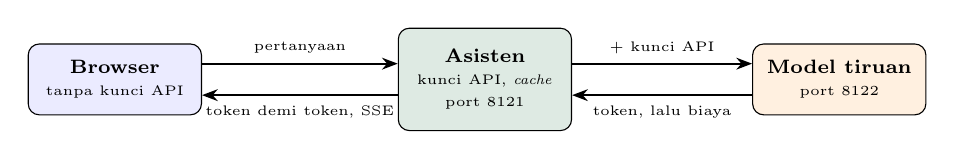
\begin{tikzpicture}[
    font=\scriptsize,
    kotak/.style={draw, rounded corners, minimum height=0.9cm,
                  minimum width=2.2cm, align=center, font=\scriptsize\bfseries},
    panah/.style={-{Stealth[length=2mm]}, thick}
  ]
    \node[kotak, fill=blue!8] (browser) at (0,0) {Browser\\{\tiny\mdseries tanpa kunci API}};
    \node[kotak, fill=praditagreen!15, minimum height=1.3cm] (asisten) at (4.7,0) {Asisten\\{\tiny\mdseries kunci API, \textit{cache}}\\{\tiny\mdseries port 8121}};
    \node[kotak, fill=orange!12] (model) at (9.2,0) {Model tiruan\\{\tiny\mdseries port 8122}};

    \draw[panah] ([yshift=0.2cm]browser.east) -- node[font=\tiny, above] {pertanyaan} ([yshift=0.2cm]asisten.west);
    \draw[panah] ([yshift=-0.2cm]asisten.west) -- node[font=\tiny, below] {token demi token, SSE} ([yshift=-0.2cm]browser.east);
    \draw[panah] ([yshift=0.2cm]asisten.east) -- node[font=\tiny, above] {+ kunci API} ([yshift=0.2cm]model.west);
    \draw[panah] ([yshift=-0.2cm]model.west) -- node[font=\tiny, below] {token, lalu biaya} ([yshift=-0.2cm]asisten.east);
  \end{tikzpicture}

  \vspace{4pt}
  {\small Browser tidak pernah berbicara langsung dengan model. Jawabannya
  kembali sebagai Server-Sent Events (SSE). Modelnya tiruan: token pertama
  0,6 detik, lalu 120 token tiap 20 ms.}
\end{frame}

\begin{frame}{{\Large Empat Skenario Pertanyaan, Diukur}}
  \vspace{6pt}
  \centering
  {\footnotesize
  \begin{tabularx}{\textwidth}{Yllll}
    \hline
    \textbf{Skenario} & \textbf{Token pertama ms} & \textbf{Selesai ms} & \textbf{Token dibayar} & \textbf{\textit{Cache}} \\
    \hline
    tanpa \textit{streaming} & 2.983,8 & 2.983,8 & 126 & MISS \\
    \hline
    \textit{streaming} & 601,7 & 3.003,4 & 127 & MISS \\
    \hline
    \textit{streaming}, kalimat sama & 0,7 & 0,7 & 0 & HIT \\
    \hline
    \textit{streaming}, kalimat lain & 602,0 & 3.000,2 & 127 & MISS \\
    \hline
  \end{tabularx}}

  \vspace{6pt}
  {\small \textit{Streaming} menyembunyikan \textit{latency}, tidak
  menghapusnya. \textit{Cache} kecocokan persis tidak mengenali makna, dan
  itulah alasan \textit{semantic cache} menjadi topik penelitian keempat.}
\end{frame}

\begin{frame}{{\Large Lima Risiko Menurut OWASP}}
  \vspace{4pt}
  \centering
  {\footnotesize
  \begin{tabularx}{\textwidth}{lY}
    \hline
    \textbf{Risiko} & \textbf{Cara meredam} \\
    \hline
    LLM01 Prompt Injection & pisahkan perintah dari data \\
    \hline
    LLM02 Sensitive Information Disclosure & jangan kirim data pribadi yang tidak dibutuhkan \\
    \hline
    LLM05 Improper Output Handling & tampilkan jawaban model lewat \texttt{textContent} \\
    \hline
    LLM06 Excessive Agency & hak sekecil mungkin, persetujuan sebelum mengubah data \\
    \hline
    LLM10 Unbounded Consumption & batasi token dan pasang \textit{rate limiting} \\
    \hline
  \end{tabularx}}

  \vspace{4pt}
  {\small Daftar dari Open Worldwide Application Security Project (OWASP)
  untuk aplikasi LLM 2025.}
\end{frame}

\section{Persiapan Latihan}

\begin{frame}{\hfill}
  \centering
  \Huge{\textbf{Persiapan Latihan}}
\end{frame}

\begin{frame}[fragile]{{\Large Hanya Python 3 dan Chrome}}
  \vspace{2pt}
\begin{lstlisting}[language=bash]
cd sources/chapter14
python3 --version
google-chrome --version

# Keluarannya:
# Python 3.15.2
# Google Chrome 157.0.8103.38
\end{lstlisting}
  \vspace{2pt}
  {\small Skrip pengukur menyalakan dan mematikan sendiri proses yang
  diukurnya. \texttt{ukur-skala.py} sengaja membebani, tetapi hanya proses
  sendiri di 127.0.0.1.}
\end{frame}

\section{Latihan 1 dan 2}

\begin{frame}{\hfill}
  \centering
  \Huge{\textbf{Latihan 1 dan 2:\\Penskalaan dan Partisi}}
\end{frame}

\begin{frame}[fragile]{{\Large Dua Kapasitas Basis Data}}
  \vspace{2pt}
\begin{lstlisting}[language=bash]
python3 ukur-skala.py
JUMLAH_KONEKSI=16 python3 ukur-skala.py

# Keluarannya, baris 4 dan 8 replika saja, 4 lalu 16 koneksi:
#   Replika  Permintaan/detik   p50 ms   p95 ms  Efisiensi
#         4             198.2    161.4    168.6        46%
#         8             198.0    161.4    168.9        23%
#
#         4             285.0    105.2    181.5        68%
#         8             347.8     87.4    143.3        41%
\end{lstlisting}
  \vspace{2pt}
  {\small Kalikan \textit{throughput} dengan p50 dalam detik, lalu bandingkan
  dengan 32 \textit{worker}.}
\end{frame}

\begin{frame}[fragile]{{\Large Dua Cara Membagi Data}}
  \vspace{2pt}
\begin{lstlisting}[language=bash]
python3 partisi.py

# Keluarannya:
#   Cara                           Pindah Terberat, kunci Terberat, permintaan
#   modulo                          80.2%           20.2%                24.3%
#   consistent hashing, 1 titik      2.1%           49.2%                43.3%
#   consistent hashing, 100 titik   20.2%           21.2%                26.9%
\end{lstlisting}
  \vspace{2pt}
  {\small Lalu ubah \texttt{JUMLAH\_NODE\_AKHIR} menjadi 8. Modulo kini hanya
  memindahkan 50,0\%, karena delapan kelipatan empat.}
\end{frame}

\section{Latihan 3, 4, dan 5}

\begin{frame}{\hfill}
  \centering
  \Huge{\textbf{Latihan 3, 4, dan 5:\\Rencana, Offline, Cold Start}}
\end{frame}

\begin{frame}[fragile]{{\Large Rencana Kapasitas dari Angka Sendiri}}
  \vspace{2pt}
\begin{lstlisting}[language=bash]
python3 rencana-kapasitas.py | tail -1

# Keluarannya:
#   Total: 28 replika, 15 node basis data, Rp 26.4 juta per bulan
\end{lstlisting}
  \vspace{4pt}
  {\small Tanpa \textit{cache} katalog: 33 \textit{node}, Rp 48,0 juta. Pada
  200 kali lipat: 55 replika, 28 \textit{node}, Rp 50,1 juta, dan 152 koneksi
  katalog per \textit{node} melewati batas 100, sehingga butuh
  \textit{pooler}.}
\end{frame}

\begin{frame}[fragile]{{\Large Mode Offline dan Cold Start}}
  \vspace{2pt}
\begin{lstlisting}[language=bash]
python3 ukur-offline.py | tail -3
# Keluarannya:
#   3, profil sama  down      8  cache     mengendalikan        31         0
#   4, profil baru  down      0  gagal     -                     -         0
#                   Chrome: net::ERR_CONNECTION_REFUSED

python3 ukur-cold-start.py | tail -2
# Keluarannya:
#   cold start                       19.069   22.248        1610
#   cold start, dengan dependensi   105.565  118.585        8911
\end{lstlisting}
  \vspace{2pt}
  {\small Tiga dependensi tambahan menaikkan \textit{cold start} menjadi
  111,941 ms.}
\end{frame}

\section{Ringkasan}

\begin{frame}{\hfill}
  \centering
  \Huge{\textbf{Ringkasan}}
\end{frame}

\begin{frame}{{\Large Ringkasan}}
  \vspace{8pt}
  \begin{itemize}
    \item Satu ke dua replika: 106,8 ke 186,6 per detik. Empat dan delapan
          berhenti di 198,2 dan 198,0, batas basis data. Dengan 16 koneksi,
          delapan replika mencapai 347,8, efisiensi 41\%.
    \item Sepuluh panggilan: 0,0012 ms sebagai fungsi, 1,4436 ms lewat HTTP.
          Modulo memindahkan 80,2\% kunci, \textit{consistent hashing} 20,2\%.
    \item Rencana 100 kali lipat: 28 replika, 15 \textit{node}, lima
          \textit{shard} untuk pesanan. \textit{Cache} katalog menghemat 18
          \textit{node}.
    \item Server \textit{down}: delapan buku tetap tampil dalam 31 ms. \textit{Cold
          start} 19,069 ms. Token pertama 601,7 ms, selesai tetap 3.003,4 ms.
    \item Tiap teknik penskalaan memindahkan \textit{bottleneck}, tidak
          menghapusnya.
  \end{itemize}
\end{frame}

\end{document}
